%Ingat, jangan lupa backup file konversibilangan.tex lalu Git Pull dulu baru ubah file baru Push (Menghindari konflik karena push bersamaan)
%Commit setiap harinya bakal dicek sapa tau ada kesalahan jadi tar dinotif lewat file ini

\section{Defenisi Konversi Bilangan}
Konversi bilangan merupakan suatu proses yang mana satu system bilangan dengan basis khusus tau tertentu akan dibuat menjadi bilangan dengan basis yang lainnya. 
Yaitu dengan cara membagikan bilangan yang desimal dengan dua dan kemudian diambil sisa pembagiannya.
caranya dengan mengalikan masing-masing bit pada bilangan dengan posisi nilainya.
\\Didalam dunia perkomputer kita dapat mengenal empat macam-macam bilangan , seperti bilangan biner,bilangan oktal, bilangan desimal , dan yang terakhir adalah bilangan hexadesimal. Bilangan biner atau binary digit (bit) sendiri merupakan bilangan yang terdiri dari 1 dan 0. Bilangan oktal sendiri merupakan bilangan yang terdiri dari 0,1,2,3,4,5,6 dan 7.
Sedangkan bilangan desimal sendiri merupakan bilangan yang terdiri dari 0,1,2,3,4,5,6,7,8 dan 9. Dan yang terakhir adalah bilangan hexadesimal yang merupakan bilangan yang terdiri dari 0,1,2,3,4,5,6,7,8,9,A,B,C,D,E dan F.

\section{Konversi bilangan biner}
\subsection{Bilangan Biner}
Sistem bilangan biner merupakan sistem dengan penulisan angka yaitu 0 dan 1.Sistem bilangan biner  modern ditemukan oleh Gittfried Wilhem Leibniz pada abad ke 17. Sistem biner juga biasa disebut dengan bit atau,Binary digit.
\subsection{Konsep Bilangan Biner}
Bilangan biner menggunakan metode yang berkaitan dengan basis,bilangan biner juga menggunakan berbasis 2. Adapun contoh biner sebagai berikut : \\
\begin{itemize}
\item 1110(2) = (1x23)+(1x22)+(1x21)+(0x20)\\
   	  = 8+4+2+0\\
             = 14  
\end{itemize}
\subsection{Konversi Sistem Bilangan Biner ke Desimal}
Bilangan Biner dapat dikonversikan ke bentuk desimal dengan cara mengalikan bit dalam bilangan dengan position valuenya.Bilangan binari 101101 dapat dikonversikan ke dalam bentuk desimal senilai :
\\  12	=110\\
1002	= 410\\
10002= 810\\
1000002 = 3210\\
----------------------+\\
101101 = 4510\\
\subsection{Konversi Sistem Bilangan Biner ke Oktal}
Cara untuk mengkonversi bilangan biner ke oktal dapat dilakukan dengan mengkonversi tiga buah digit biner.

\subsection{Konversi Bilangan Biner ke Bilangan Hexadesimal}
Konversi bilangan biner ke bilangan hexadesimal hampir mirip seperti Konversi pada bilangan oktal. Hanya saja pada bilangan hexadesimal memakai 4 digit angka yang diambil dari bilangan biner.Selain itu untuk nilai yang lebih besar dari 9 dapat diganti dengan huruf Heksadesimal seperti A,B,C,D sampai H. 
\section{Bilangan Oktal} %Septia Rahayu (26-10-2017)
Bilangan oktal adalah sistem bilangan yang berbasis 8 dan mempunyai delapan simbol bilangan yang berbeda : 0,1,2,...,7.
\\
	Teknik pembagian yang berurutan dapat menggunakan untuk mengubah bilangan desimal menjadi bilangan oktal. Bilangan desimal yang akan diubah secara berturut-turut dibagi dengan 8 dan sisa pembagian harus selalu dicatat. Sebagai contoh, untuk mengubah bilangan 5819.10 ke oktal.
\subsection{Konversi Oktal ke Desimal}
Cara untuk mengkorvesikan bilangan oktal ke heksadesimal yaitu dengan mengkonveksikan bilangan oktal tersebut ke biner terlebih dahulu kemudian bilangan tersebut di konveksikan ke heksadesimal. Untuk lebih jelasnya, perhatikan contoh konveksi bilangan oktal ke heksadesimal sebagai berikut:
\\	Contoh konversi oktal ke heksadesimal:
\\357(8)=......(16) 357 oktal sama dengan berapa bilangan heksadesimal?
\\Adapun cara pengerjaannya sebagai berikut adalah:
\begin{enumerate}
	\item Kita pisahkan 357 menjadi 3, 5, dan 7 kemudian konversikan ke biner 
	\item 3 = 011		5=101		7=111
	\item Setelah dapat biner nya yaitu 011101111 kemudian konversi biner tersebut ke heksadesimal. 
	\item 011101111  -------- 1111 = 15 = F            1110 = 14 = E       0 = 0
	\item Maka di dapat bahwa 357 oktal sama dengan EF hexadesimal	
\end{enumerate}



\section{Bilangan Desimal} Salwaa Tania (26-10-2017)
Bilangan desimal adalah bilangan yang menggunakan 10 angka mulai 0 sampai 9 berturut-turut. Setelah angka 9 , maka angka berikutnya adalah 10,11,12 dan seterusnya. Bilangan desimal disebut juga dengan bilangan berbasis 10.
\\Contoh: 1710
\\Berikut bagaimana cara melakukan konversi antar basis bilangan: 
\begin{itemize}
	\item Cara Konversi desimal ke basis lainnya
	\item Konversi desimal ke biner
	\item Konversi desimal ke Oktal
	\item Konversi desimal ke Heksadesimal
\end{itemize}
\subsection{Cara mengkoversikan bilangan desimal ke biner}
\begin{figure}[ht]
\centerline{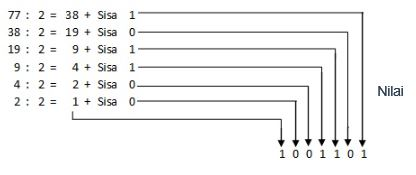
\includegraphics[width=1\textwidth]{figures/konversibiner.JPG}}
\caption{Cara mengkonversikan bilangan desimal ke biner}
\label{Contoh Konversi Bilangan Desimal}
\end{figure}
Seperti yang bisa kita lihat pada \ref{konversibiner} bahwa cara mengkonversikan bilangan desimal ke dalam bilangan biner adalah dengan membagi bilangan desimal dengan nilai 2 (basis). Cara ini merupakan cara yang sering digunakan oleh banyak orang dan cara ini cukup mudah untuk di pahami dan diterapkan. Hasil yang di dapat dari perhitungan \ref{konversibiner} adalah bilangan desimal 77 = 1001101 (bilangan biner). Dengan menggunakan rumus perhitungan konversi tersebut, kita bisa lihat langkah – langkah nya seperti berikut ini : 
\begin{enumerate}
	\item Pertama kita bagi 77 dengan 2, didapat bilangan bulat hasil bagi adalah 39 dengan sisa hasil bagi adalah 1,atau dengan kata lain 77=2*(36+1)
	\item Selanjutnya bilangan bulat hasil bagi tersebut (36) kita bagi dengan 2 lagi, 36/2=18,sisa hasil bagi 0
	\item Ulangi lagi langkah tersebut sampai bilngan bulat hasil bagi sama dengan 0. Setelah itu tulis sisa hasil bagi mulai dari bawah ke atas
	\item Barulah kita mendapatkan hasil bahwa bilangan desimal 77 adalah bilangan desimal dari bilangan biner 1001110.
\end{enumerate}
\subsection{Cara mengkonversikan bilangan desimal ke oktal
Dengan rumus yang sama seperti biner kita bisa  lakukan juga untuk bilangan berbasis 8(oktal).
\\Langkah - langkah :
\begin{enumerate}
	\item Pertama-tama 67/8=8, sisa 3
	\item Lalu 8/8=0,sisa 0
	\item Terakhir 1/8=0 sisa 1
	\item Dengan demikian dari hasil perhitungan di dapatkan 6710=1038
	\item Kita juga dapat menggunakan fungsi microsoft excel DEC20CT() untuk konversi bilngan desimal ke oktal.
\end{enumerate}
\section{Bilangan Heksadesimal}
Bilangan heksadesimal, atau bilangan heksa, atau bilangan basis 16, adalah sebuah sistem bilangan yang menggunakan 16 simbol.
\begin{figure}[ht]
\centerline{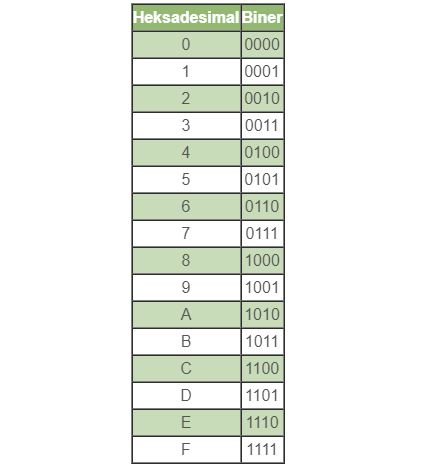
\includegraphics[width=1\textwidth]{figures/konversiheksa.JPG}}
\caption{Tabel Konversi Bilangan Heksadesimal ke Biner}
\label{Tabel Konversi}
\end{figure}
Berbeda dengan sistem bilangan desimal, bisa di lihat pada \ref{konversiheksa} simbol yang digunakan dari sistem ini menggunakan 16  buah simbol, mulai dari 0 sampai 9, kemudian dilanjut dari A sampai F. Jadi, angka A sampai F merupakan simbol untuk 10 sampai 15. Contoh penulisan : C516.
Untuk dapat mengetahui bagimana cara mengubahnya antara bilangan satu dengan yang lain. Sebenarnya pada dasarnya, bilangan heksadesimal digunakan sebagai salah satu cara untuk menampilkan informasi bilangan biner dalam deret yang lebih pendek.
\subsection{Konversi Bilangan Heksadesimal Ke Oktal}
Untuk konversi Bilangan Heksadesimal ke Oktal lebih mudahnya digunakan sebuah perantara, yaitu konvensi bilangan heksadesimal kepada bilangan biner lalu Bilangan biner kepada Bilangan oktal.
Konversi ini Juga dapat dilakukan dengan menggunakan Program Excel, seperti LibreOffice yang bernama LibreOffice-Calc dengan Rumus seperti berikut :  "=HEX2OCT( 'kolom' )".
\subsection{Konversi Bilangan Heksadesimal ke Desimal}
Cara untuk mengkonversi bilangan heksadesimal kedalam bentuk bilangan desimal terdapat dua cara yaitu dengan mengunakan perhitungan manual yaitu dengan cara mengalikan masing-masing bit dalam bilangan dengan position valuenya.
Langkah-langkah :
\begin{itemize}
\item Digit-digit dipisahkan. Dan jika terdapat huruf A-F menggantinya dengan bilangan desimal padananya
\item Mengalikan dari tiap digit terhadap nilai tempatnya.
\begin{itemize}
\section{Bilangan Desimal} Salwaa Tania (26-10-2017)
Bilangan desimal adalah bilangan yang menggunakan 10 angka mulai 0 sampai 9 berturut-turut. Setelah angka 9 , maka angka berikutnya adalah 10,11,12 dan seterusnya. Bilangan desimal disebut juga dengan bilangan berbasis 10.
\\Contoh: 1710
\\Berikut bagaimana cara melakukan konversi antar basis bilangan: 
\begin{itemize}
	\item Cara Konversi desimal ke basis lainnya
	\item Konversi desimal ke biner
	\item Konversi desimal ke Oktal
	\item Konversi desimal ke Heksadesimal
\end{itemize}
\subsection{Cara mengkoversikan bilangan desimal ke biner}
\begin{figure}[ht]
\centerline{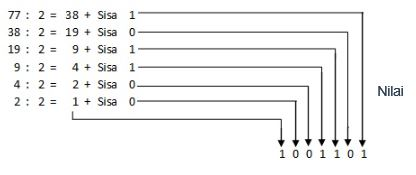
\includegraphics[width=1\textwidth]{figures/konversibiner.JPG}}
\caption{Cara mengkonversikan bilangan desimal ke biner}
\label{Contoh Konversi Bilangan Desimal}
\end{figure}
Seperti yang bisa kita lihat pada \ref{konversibiner} bahwa cara mengkonversikan bilangan desimal ke dalam bilangan biner adalah dengan membagi bilangan desimal dengan nilai 2 (basis). Cara ini merupakan cara yang sering digunakan oleh banyak orang dan cara ini cukup mudah untuk di pahami dan diterapkan. Hasil yang di dapat dari perhitungan \ref{konversibiner} adalah bilangan desimal 77 = 1001101 (bilangan biner). Dengan menggunakan rumus perhitungan konversi tersebut, kita bisa lihat langkah – langkah nya seperti berikut ini : 
\begin{enumerate}
	\item Pertama kita bagi 77 dengan 2, didapat bilangan bulat hasil bagi adalah 39 dengan sisa hasil bagi adalah 1,atau dengan kata lain 77=2*(36+1)
	\item Selanjutnya bilangan bulat hasil bagi tersebut (36) kita bagi dengan 2 lagi, 36/2=18,sisa hasil bagi 0
	\item Ulangi lagi langkah tersebut sampai bilngan bulat hasil bagi sama dengan 0. Setelah itu tulis sisa hasil bagi mulai dari bawah ke atas
	\item Barulah kita mendapatkan hasil bahwa bilangan desimal 77 adalah bilangan desimal dari bilangan biner 1001110.
\end{enumerate}


\section{Fungsi dari Konversi Bilangan} %Luthfi Muhammad Nabil (25-10-2017)
Membuat sebuah program tidak hanya membutuhkan bahasa pemrograman. Pada bagian komputernya juga memerlukan sebuah bahasa yang dimengerti oleh komputer tersebut. yaitu bilangan biner. jadi salah satu Fungsi dari konversi bilangan ini salah satunya adalah untuk membuat sebuah program. Selain menggunakan bilangan desimal yang biasa kita temui di keseharian kita, pembuatan sebuah program itu terkadang juga menggunakan bilangan biner, oktal, dan hexadesimal.
Fungsi lain dari Konversi bilangan ini salah satunya adalah untuk membaca sebuah perintah yang dimana perintah tersebut masih menggunakan perintah yang hanya bisa dibaca oleh komputer yaitu Biner. tetapi dengan adanya Konversi Bilangan, Sebuah angka tersebut bisa dijadikan sebagai suatu line perintah bahkan sebuah kata yang nantinya dapat dimunculkan oleh komputer kepada pengguna. Pembuatan aplikasi sendiri membutuhkan sebuah Konversi Bilangan yang nantinya akan menggerakan sebuah modul - modul dalam sebuah perangkat yang dipakai dalam aplikasi tersebut. 
Konversi Sendiri dilakukan dalam sebuah Processor atau ALU yang mereka hanya dapat membaca kode biner yang nantinya saat setelah diproses akan dimasukan ke memori yang nanti akan dikonversi ditampilkan ke layar dengan berbentuk yang sesuai dengan yang dibutuhkan
\\Membuat sebuah program tidak hanya membutuhkan bahasa pemrograman. Pada bagian komputernya juga memerlukan sebuah bahasa yang dimengerti oleh komputer tersebut. yaitu bilangan biner. jadi salah satu Fungsi dari konversi bilangan ini salah satunya adalah untuk membuat sebuah program. Selain menggunakan bilangan desimal yang biasa kita temui di keseharian kita, pembuatan sebuah program itu terkadang juga menggunakan bilangan biner, oktal, dan hexadesimal.
\\Fungsi lain dari Konversi bilangan ini salah satunya adalah untuk membaca sebuah perintah yang dimana perintah tersebut masih menggunakan perintah yang hanya bisa dibaca oleh komputer yaitu Biner. tetapi dengan adanya Konversi Bilangan, Sebuah angka tersebut bisa dijadikan sebagai suatu line perintah bahkan sebuah kata yang nantinya dapat dimunculkan oleh komputer kepada pengguna. Pembuatan aplikasi sendiri membutuhkan sebuah Konversi Bilangan yang nantinya akan menggerakan sebuah modul - modul dalam sebuah perangkat yang dipakai dalam aplikasi tersebut. 

\section{Penerapan Konversi Bilangan} %Luthfi Muhammad Nabil (26-10-2017)
Konversi Bilangan diterapkan khususnya pada bidang Teknologi. Selain sebagai instruksi, Konversi sendiri dapat dikenal sebagai pengenal dalam situasi tertentu. seperti untuk mengenal warna dan sebagainya. Beberapa contoh dari penerapan tersebut adalah sebagai berikut : 
\begin{itemize}
	\item Sebagai kode warna dalam pemrograman \\ Konversi Bilangan sering sekali dipakai untuk mengetahui berapa tingkat warna dan seberapa pekat warna tersebut. Konversi Bilangan pada kasus ini menggunakan Konversi Desimal ke Heksadesimal dimana warna terbagi menjadi Merah, Hijau, Biru. 
	\item Sebagai Penampil Angka dalam Kalkulator \\ Dengan adanya Konversi Bilangan, Angka yang dikirimkan ke memori akan diubah kedalam bentuk angka biner yang sebelumnya dikonversi dengan menekan sebuah tombol yang mengirimkan aliran kepada memori untuk mengirimkan angka biner.	
\end{itemize}

\section{Rangkuman} %Luthfi Muhammad Nabil (28-10-2017)
Konversi Bilangan adalah Konversi dimana sebuah bilangan akan dikonversikan menjadi tipe bilangan yang lain. Tipe bilangan sendiri cukup beragam, seperti Bilangan Biner, Desimal, Oktal, dan Heksadesimal. Cara pengonversiannya sendiri bermacam ? macam, ada yang mampu langsung dikonversikan menjadi bilangan tipe tujuan atau diubah terlebih dahulu ke bilangan decimal. Pemakaian dari Konversi Bilangan pun beragam. Dimulai dari proses hitungan pada kalkulator dan ALU sampai pembacaan kode pada kode Heksadesimal di computer. 
\\Pada dasarnya Konversi bilangan memiliki beberapa fungsi baik dalam Komputer maupun diluar computer. Dengan adanya metode ini kita diharapkan dapat membaca dan mengkonversi sebuah instruksi kedalam computer yang dapat terbaca oleh computer lalu dapat dikonversikan ke dalam bentuk sebuah bilangan yang kita inginkan. Bahkan seseorang yang buta warna dapat melihat warna yang tidak bisa dia lihat dengan kode yang telah tersedia yaitu kode warna. 
%Note : Setiap mau push kasih note atau attention biar diarahkan supaya sebelum push nanti di pull dulu biar tau siapa yang mau push (Komunikasi Tetap Terjaga)
%Untuk konversi bilangan desimal ada penyesuaian jadi agak lebih mendetail (Salwaa Tania)

%Antara hari sabtu/minggu/senin bakal disusun jadi struktur bakal berubah
